\documentclass{article}
\usepackage{amsmath}
\usepackage{amssymb}
\usepackage{bm}
\usepackage{amsthm}
\usepackage{enumerate}
\usepackage{graphicx}
\usepackage{psfrag}
\usepackage{color}
\usepackage{url}
\usepackage{listings}
\usepackage{xcolor}
\usepackage{tikz}
\usepackage{mdframed}
\usepackage{multirow}
\usepackage{tikz-qtree}
\usepackage[utf8]{inputenc}
\usetikzlibrary{positioning}
\tikzset{main node/.style={circle,fill=gray!20,draw,minimum size=.5cm,inner sep=0pt},}

% In line code stuff%
\definecolor{codegreen}{rgb}{0,0.5,0}
\definecolor{codewhite}{rgb}{1,1,1}
\definecolor{codegray}{rgb}{0.85,0.85,0.85}
\definecolor{codepurple}{rgb}{0.58,0,0.82}
\definecolor{codeblack}{rgb}{0,0,0}
\definecolor{codeorange}{rgb}{0.8,0.4,0}

\lstdefinestyle{mystyle}{
    backgroundcolor=\color{codegray},   
    commentstyle=\color{codegray},
    keywordstyle=\color{codegreen},
    numberstyle=\color{codegray},
    stringstyle=\color{codeorange},
    basicstyle=\ttfamily ,
    breakatwhitespace=false,         
    breaklines=true,                 
    captionpos=b,                    
    keepspaces=true,                 
    numbers=left,                    
    numbersep=5pt,                  
    showspaces=false,                
    showstringspaces=false,
    showtabs=false,                  
    tabsize=4
}
\lstset{style=mystyle}
\setlength{\hoffset}{-1in}
\addtolength{\textwidth}{1.5in}
\setlength{\voffset}{-1in}
\addtolength{\textheight}{1.5in}

% Custom commands%
\newcommand{\be}{\begin{enumerate}}
\newcommand{\ee}{\end{enumerate}}
\newcommand{\BigO}[1]{\ensuremath\mathcal{O}\left(#1\right)}
\newcommand{\il}[1]{\lstinline!#1!}
\newcommand{\norm}[1]{\left|\left|#1\right|\right|}
\newcommand{\abs}[1]{\left|#1\right|}
\newcommand{\parens}[1]{\left(#1\right)}
\newcommand{\bracks}[1]{\left\{#1\right\}}
\newcommand{\sqbracks}[1]{\left[#1\right]}
\newcommand{\vep}{\varepsilon}
\newcommand{\ceiling}[1]{\left\lceil#1\right\rceil}
\newcommand{\R}{\mathbb{R}}
\newcommand{\N}{\mathbb{N}}
\newcommand{\Z}{\mathbb{Z}}
\newcommand{\F}{\mathbb{F}}
\newcommand{\A}{\mathcal{A}}
\newcommand{\distrib}[2]{\text{#1}\left(#2\right)}
\newcommand{\dd}[1]{\frac{d}{d#1}}
\newcommand{\abracks}[1]{\left< #1\right>}

\newenvironment{answer}
    {\begin{mdframed}[
    backgroundcolor=lightgray,
    outerlinewidth=0
    ]\emph{Answer.} }
    {\end{mdframed}}

\newenvironment{centeredtable}[1]
    {\begin{center}
    \begin{tabular}{#1}}
    {\end{tabular} 
    \end{center}
    }

\begin{document}
	\begin{center}
		\textbf{Fall 2020, Math 693A:\ Project Report} \\
		\textbf{Due:\ December 9th, 2020} \\
		\textbf{Joseph Diaz: 819947915}
	\end{center}
\noindent\makebox[\linewidth]{\rule{\paperwidth}{0.4pt}}
\section*{Introduction}
Discrete Optimization is an almost entirely different beast from the calculus inspired
Numerical Optimization that we delve into in this course. 
As such, the methods by which discrete problems are solved are very different from the 
likes of line search, trust region and gradient descent. \\\\

\noindent
In many discrete optimizations problems it is possible, at least in 
principle,
to come up with a means of generating all possible states of a problems and checking for
which represents the best solution. In practice, however, this is usually impossible.
As these states could be so 
\textit{numerous} that it would take far too long to generate and check each, and very 
likely 
there isn't enough space in any computer's RAM to store them all.
These 2 issues taken together lead to the development of... \\\\

\noindent
Branch and Bound, whose method was originally described in [1], is an algorithm design
paradigm with applications in Discrete Optimization and
Combinatorial Optimization in which the following are employed
\begin{itemize}
    \item A set of possible solutions is generated by a state space search.
    \item A means of recursively splitting the solution set into subsets.
    \item A method for determining if any of these subsets has a viable solution, or 
    if it should be cut from the search space. 
\end{itemize}

\section*{Methods}
This set $S_1$ of possibles solutions, and its subsets, are usually represesented as a 
binary tree; where $S_1$ is the root and each pair of child nodes are disjoint subsets of 
the parent they belong to. So in general, the relationship between $S_1$ and the other nodes 
is the following recursive relation:
$$\forall i \in \mathbb{N}, S_i = S_{2i} \cup S_{2i+1},
S_{2i} \cap S_{2i+1} = \varnothing$$

\begin{center}
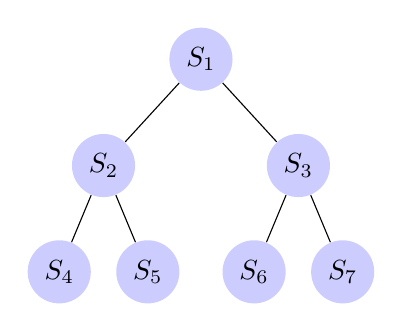
\begin{tikzpicture}  
    [scale=.9,auto=center,every node/.style={circle,fill=blue!20}] 
    % here, node/.style is the style pre-defined, that will be the default layout of all the nodes. You can also create different forms for different nodes.  
        
    \node (a1) at (0,0) {$S_1$};
    \node (a2) at (-1.375,-1.5) {$S_2$};
    \node (a3) at (1.375,-1.5) {$S_3$};
    \node (a4) at (-2,-3) {$S_4$};
    \node (a5) at (-.75,-3) {$S_5$};
    \node (a6) at (.75,-3) {$S_6$};
    \node (a7) at (2,-3) {$S_7$};
    
    
    \draw (a1) -- (a2); % these are the straight lines from one vertex to another  
    \draw (a1) -- (a3);  
    \draw (a2) -- (a4);  
    \draw (a2) -- (a5);  
    \draw (a3) -- (a6);  
    \draw (a3) -- (a7);  
    
\end{tikzpicture}
\end{center}

\noindent
This splitting of the solution set and tree representation is what 
gives us the ``branching'', but where does the bounding come in?
Instead of following each branch down to a leaf and comparing these solutions, we 
employ a schema to determine which branches are worth traversing and which aren't.
Most Branch and Bound algorithms rely on 2 different bounds that need to be computed 
using each node of tree:\\\\

\noindent
\textbf{Optimistic Bound} - The lower (or upper, if you're maximizing) bound of all 
possible solutions represented by a given node. A quick, efficient, and accurate 
calculation of this bound is crucial if you're expecting your algorithm to get anywhere.
\\\\

\noindent
\textbf{Pessimistic Bound} - The best solution to the optimization problem so far. 
Comparison between this and the optimistic bound on newly visited node is the primary 
decision maker for disregarding a branch or exploring it further.\\\\

\noindent
Given an objective function $f(x)$ for $x \in \Omega$ and $S_1 \subset \Omega$ a set
of possible solutions. \\
\begin{itemize}
    \item[1.] Using a heuristic, locate a solution $x_h$ and store $S = f(x_h)$ or 
    $S= \infty$ if no such $x_h$ exists. $S$ will also denote best solutions found
    so far, and will serve as the pessimistic bound to compare future solutions to.
    \item[2.] Initialize a data structure of nodes representing sets of possible solutions.
    \item[3.] Take a node $S_i$ from the data structure.
    \begin{itemize}
        \item If it represents a single solution $x$
        and $f(x) < S$, store $S = f(x)$.
        \item Otherwise, branch on $S_i$ to obtain $S_{2i}$ and $S_{2i+1}$.
        \begin{itemize}
            \item If the optimistic bound on either node is greater than $S$, discard that node.
            \item Otherwise, store the node in the data structure.
        \end{itemize}
    \end{itemize}
    \item[4.] Repeat 3 until the data structure is empty.
\end{itemize}

\noindent
Choice of Data Structure can impact the utility and ``behavior'' of the algorithms 
itself:
\begin{itemize}
    \item Queue - Yields behavior similar to a ``breadth first'' search. As in, all 
    nodes on a given level are examined before going down a branch.
    \item Stack - Yields behavior similar to a ``depth first'' search, where-in each 
    branch is explored to it's exhaustion before examining other nodes.
    \item Priority Queue - If each node is sorted by it's bound, then this structure 
    gives a ``best first'' sort of search where the most promising branches are 
    explored first.
\end{itemize}
\section*{Results}
Here we examine the performance of a branch and bound style algorithm on a 
problem of discrete resource management: The One-Dimensional Knapsack Problem.\\\\
\textbf{The Knapsack Problem} - Given a collection of items, each with a weight and 
a value; which items should you take such that the overall value of the items taken is
maximized, subject to the maximum weight that you can carry in your knapsack? \\\\
The problem itself is very old, but the name is often attributed to the
American Mathematician Tobias Dantzig. This problem is NP-Complete, and so no 
polynomial time algorithm for solving the problem exists. This complexity and the 
decision tree associated with inclusion and exclusion of set elements makes Branch and 
Bound an ideal approach for tackling this thorny problem.\\\\
As a means of measuring how well the problem is solved by Branch and Bound, the graph 
on the next page shows the $\log_{10}$ of the number of 
iterations of the algorithm to find the 
optimal solution against the total number of items considered for the problem. Each 
run of the program generates $n$ items with values taken from $\distrib{Unif}{10, 20}$, 
weights from $\distrib{Unif}{1,5}$ and with a max weight for the problem taken from 
$\distrib{Unif}{n/2, 3n/4}$ (here ``Unif'' represents a uniform distribution). 


\begin{center}
\includegraphics[width=\linewidth]{BnBalone.jpg}
\end{center}
As stated at the top, this problem could, in principle, be solved by generating every 
possible subset of the $n$ items, filtering out the arrangements that don't satisfy the
weight limit, and choosing the one of greatest values remains. In practice, however, 
this won't work. 

\begin{center}
\includegraphics[width=\linewidth]{ForceVsBound.jpg}
\end{center}
The number of the subsets of $n$ items is $\sim 2^n$ subsets; this number is 
calculable by most modern computer for $\log_{10} n < 4$, but even for $n$ as
low as 99, $2^n \sim 6 \times 10^{29}$. If a schema was devised that 
could generate a billion unique arrangements every second, it would still take 
$\sim 10^{22}$ years to generate all $2^n$ subsets. The graph on the bottom of 
the previous page illustrates this vast difference in the number of iteration 
to guarantee an optimal solution.  
\section*{Conclusion}
Branch and Bound is the most common algorithm paradigm in use for solve NP-Hard 
optimization problems; like the Travelling Salesmen Problem for example. Indeed, many 
other examples of NP-Hard and NP-Complete problems only have reasonable solutions using
similar methods. In fact, some generalizations of the algorithm effectively subsume 
other well known search algorithms like A* and B* [2].

\subsection*{References}
\be[1.]
    \item Land, A. H., and A. G. Doig. ``An Automatic Method of Solving Discrete 
    Programming Problems.'' Econometrica 28, no. 3 (1960).
    \item Nau, Dana S., Kumar, Vipin, Kanal, Laveen. ``General branch and bound, and 
    its relation to A* and AO*.'' Artificial Intelligence 23 (1984)
\ee

\noindent\makebox[\linewidth]{\rule{\paperwidth}{0.4pt}}
	
\end{document}
